\documentclass[12pt, a4paper, titlepage, table]{article}
\usepackage{pdfpages}
\usepackage[utf8]{inputenc}
\usepackage[T1]{fontenc}
\usepackage{titlesec}
\usepackage[french]{babel}
\usepackage{caption}
\usepackage{float}
\usepackage{graphicx}
\usepackage[inner=2cm, outer=2cm, top=2cm, bottom=2cm]{geometry}
\usepackage[T1]{fontenc}
\usepackage{times}
\usepackage{xr} 
\usepackage{multirow}
\usepackage{amsmath}
\usepackage{array}
\usepackage{booktabs}
\usepackage{tabularx}
\usepackage{ragged2e}
\usepackage{adjustbox}

\begin{document}
	\label{document}
	\title{Etude de l'insertion professionnelle des diplômés de l'université (DUT, Licence Pro, MASTER LMD et Master ENS)}
	\author{Sébastien Mertès}
	\date{\today}
	\maketitle
	\renewcommand{\thesection}{\arabic{section}.}
	\renewcommand{\thesubsection}{\thesection\arabic{subsection}}
	\renewcommand{\tablename}{Tableau}
	\renewcommand{\abstractname}{Résumé}
	\captionsetup[table]{font={small}}
	\setlength{\parindent}{0pt}
	\captionsetup{labelfont=bf, font=small}
	\tableofcontents
	\newcolumntype{C}{>{\RaggedRight\arraybackslash}X}
	\newpage
	
\section{Introduction}
	
\section{Présentation des données}
	Nous avons 3 jeux de données représentant respectivement les informations concernant l'évaluation de l'insertion professionnelle sur le marché du travail des diplômés universitaires en DUT, Licence Professionnelle, Master LMD (Licence-Master-Doctorat) et Master ENS (Enseignement) de toutes les disciplines. 
	
	Ces données ont été collectées 18 mois et 30 mois après l'obtention du diplôme des sessions  2013 à 2019. Ainsi l'enquête a commencé en décembre 2015, pour s'achever en décembre 2021.
	
	Les données collectées regroupent, par niveau de diplôme, les disciplines, le taux d'insertion, le salaire brut et net estimé, le pourcentage des types de contrat professionnel (CDI, CDD, intérimaire etc...) ainsi que les secteurs d'activité, les professions et le type d'entreprises.
	
	Les tableaux 1 à 5 décrivent les différentes variables utilisées pour cette étude.
	
\newpage

\begin{table}[H]
	\centering
	\begin{adjustbox}{max width=\textwidth}
		\begin{tabularx}{\linewidth}{|l|C|}
			\hline
			\multicolumn{1}{|c|}{\textbf{Diplôme}} & \multicolumn{1}{c|}{\textbf{Définition}} \\
			\hline
			DUT & Diplôme Universitaire de Technologie. Formation de 2 ans axée sur des compétences techniques et pratiques. \\
			\hline
			LICENCE PRO & Licence professionnelle. Programme de 1 an après un DUT ou une Licence, offrant une spécialisation professionnelle. \\
			\hline
			MASTER ENS & Master Enseignement. Diplôme permettant de devenir enseignant dans le système éducatif français. \\
			\hline
			MASTER LMD & Système européen d'enseignement supérieur avec niveaux de Licence, Master et Doctorat. \\
			\hline
		\end{tabularx}
	\end{adjustbox}
	\caption{Nom de la variable catégorielle et ses modalités concernant les diplômes universitaires}
	\label{tab:diplomes}
\end{table}

\begin{table}[H]
	\centering
	\begin{tabularx}{\textwidth}{|C|}
		\hline
		\multicolumn{1}{|c|}{\textbf{Disciplines}} \\
		\hline
		Ensemble Licence professionnelle \\
		\hline
		Autres sciences humaines et sociales \\
		\hline
		Autres formations juridiques, économiques et de gestion \\
		\hline
		Sciences de la vie et de la terre \\
		\hline
		Ensemble formations juridiques, économiques et de gestion \\
		\hline
		Psychologie \\
		\hline
		Information communication \\
		\hline
		Ensemble des départements d'IUT \\
		\hline
		Lettres, langues, arts \\
		\hline
		Sciences de l'ingénieur \\
		\hline
		Histoire-géographie \\
		\hline
		Droit \\
		\hline
		Informatique \\
		\hline
		Gestion \\
		\hline
		Sciences fondamentales \\
		\hline
		Ensemble sciences humaines et sociales \\
		\hline
		Ensemble sciences, technologies et santé \\
		\hline
		Autres sciences, technologies et santé \\
		\hline
		Économie \\
		\hline
		Ensemble Masters LMD (hors Masters enseignement et hors Dauphine et Antilles-Guyane) \\
		\hline
		Sciences de l'ingénieur \\
		\hline
		Masters enseignement \\
		\hline
		Ensemble Masters LMD (hors Masters enseignement) \\
		\hline
	\end{tabularx}
	\caption{Variable catégorielle concernant les disciplines pour les 3 niveaux de diplôme et leurs modalités}
	\label{tab:disciplines}
\end{table}

\begin{table}[H]
	\centering
	\begin{tabularx}{\textwidth}{|X|}
		\hline
		\textbf{Type de contrat} \\
		\hline
		Prof. libérale, indépendant, chef d’entreprise \\
		\hline
		Fonctionnaire \\
		\hline
		CDI \\
		\hline
		CDI de chantier ou CDI de mission \\
		\hline
		Contrat spécifique au doctorat \\
		\hline
		CDD \\
		\hline
		Vacataire \\
		\hline
		Intérimaire \\
		\hline
		Intermittent du spectacle \\
		\hline
		Contrat de professionnalisation \\
		\hline
		Emplois aidés (Contrat Initiative Emploi…) \\
		\hline
		Volontariat international \\
		\hline
	\end{tabularx}
	\caption{Variables quantitatives (\%) concernant le type de contrat}
	\label{tab:variables_sans_numeros}
\end{table}

\begin{table}[H]
	\centering
	\begin{tabularx}{\textwidth}{|X|}
		\hline
		\textbf{Type d'entreprise} \\
		\hline
		Vous-même \\
		\hline
		La fonction publique (d'etat, territoriale ou hospitalière) \\
		\hline
		Une entreprise privée \\
		\hline
		Une entreprise publique \\
		\hline
		Une association \\
		\hline
		Une personne exerçant une profession libérale ou un indépendant \\
		\hline
		Organisation internationale ou une institution de l'Union européenne \\
		\hline
		Société d'économie mixte \\
		\hline
		Un particulier \\
		\hline
	\end{tabularx}
	\caption{Variables quantitatives (\%) concernant les différents types d'entreprise}
	\label{tab:variables_liste2}
\end{table}

\begin{table}[H]
	\centering
	\begin{tabularx}{\textwidth}{|X|}
		\hline
		\textbf{Secteur d'activité} \\
		\hline
		Agriculture, sylviculture et pêche \\
		\hline
		Industries (manufacturières,  extractives et autres) \\
		\hline
		Construction \\
		\hline
		Activités immobilières \\
		\hline
		Commerce, transports, héberg-ement et restauration \\
		\hline
		Information et communication \\
		\hline
		Activités financières et d’assurance \\
		\hline
		Activités spécialisées, scientifiques et techniques \\
		\hline
		Activités de services administratifs et de soutien \\
		\hline
		Enseignement \\
		\hline
		Administration publique (hors ens.) \\
		\hline
		Santé humaine et action sociale \\
		\hline
		Arts, spectacles et activités récréatives \\
		\hline
		Autres activités de service \\
		\hline
	\end{tabularx}
	\caption{Variables quantitatives (\%) concernant les secteurs d'activité}
	\label{tab:variables_liste3}
\end{table}

\begin{table}[H]
	\centering
	\begin{tabularx}{\textwidth}{|X|}
		\hline
		\textbf{Profession} \\
		\hline
		Agriculteur \\
		\hline
		Artisan, commerçant, chef d'entreprise \\
		\hline
		Profession libérale \\
		\hline
		Personnel de catégorie A de la fonction publique \\
		\hline
		Ingénieur, cadre, prof. libérales, prof. intellectuelles sup \\
		\hline
		Personnel de catégorie B de la fonction publique \\
		\hline
		Emploi de niveau intermédiaire : technicien, agent de maîtrise… \\
		\hline
		Personnel de catégorie C de la fonction publique \\
		\hline
		Manœuvre, ouvrier \\
		\hline
		Employé de bureau, de commerce, personnel de service \\
		\hline
	\end{tabularx}
	\caption{Variables quantitatives (\%) concernant les différentes professions}
	\label{tab:variables_liste4}
\end{table}

\section{Proportion des contrats après l'obtention du diplôme}

\begin{figure}[H]
	\centering
	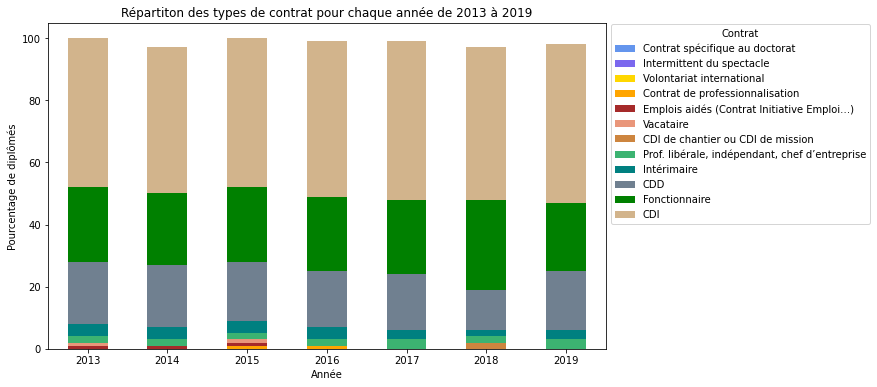
\includegraphics[width=1\textwidth]{../graphs/repartition_contrats_global.png}
	\captionof{figure}{\textbf{Répartition globale des contrats après l'obtention du diplôme}}
\end{figure}

\begin{figure}[H]
	\centering
	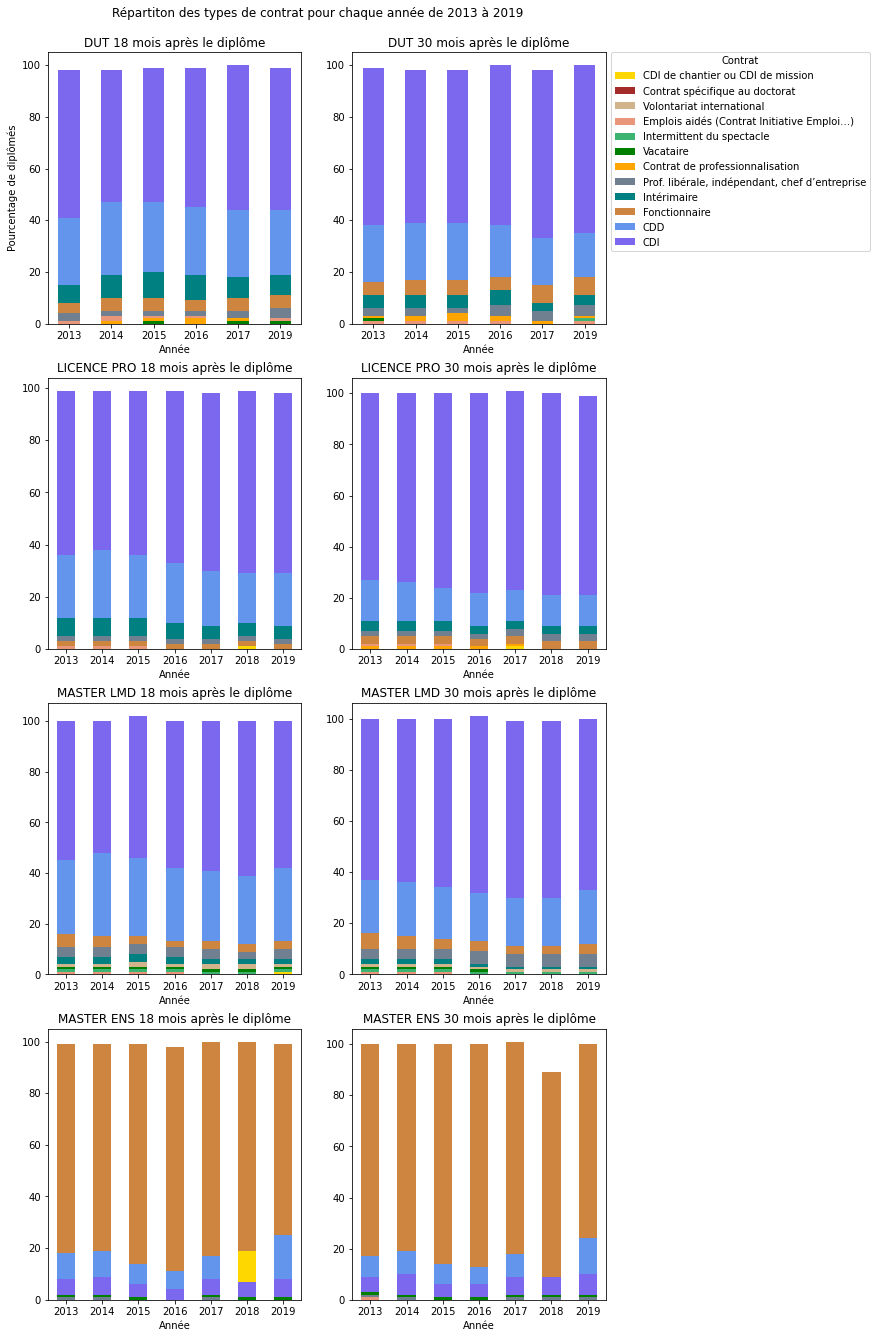
\includegraphics[width=1\textwidth]{../graphs/repartition_contrats_situation.png}
	\captionof{figure}{\textbf{Répartition des contrats à 18 et 30 mois après l'obtention du diplôme}}
\end{figure}

\section{Proportion des professions}
\begin{figure}[H]
	\centering
	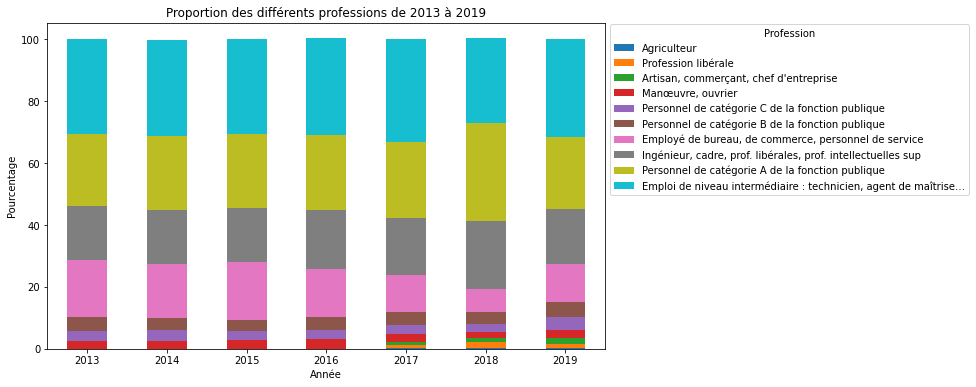
\includegraphics[width=1\textwidth]{../graphs/repartition_professions_global.png}
	\captionof{figure}{\textbf{Répartition des professions globale après l'obtention du diplôme}}
\end{figure}

\begin{figure}[H]
	\centering
	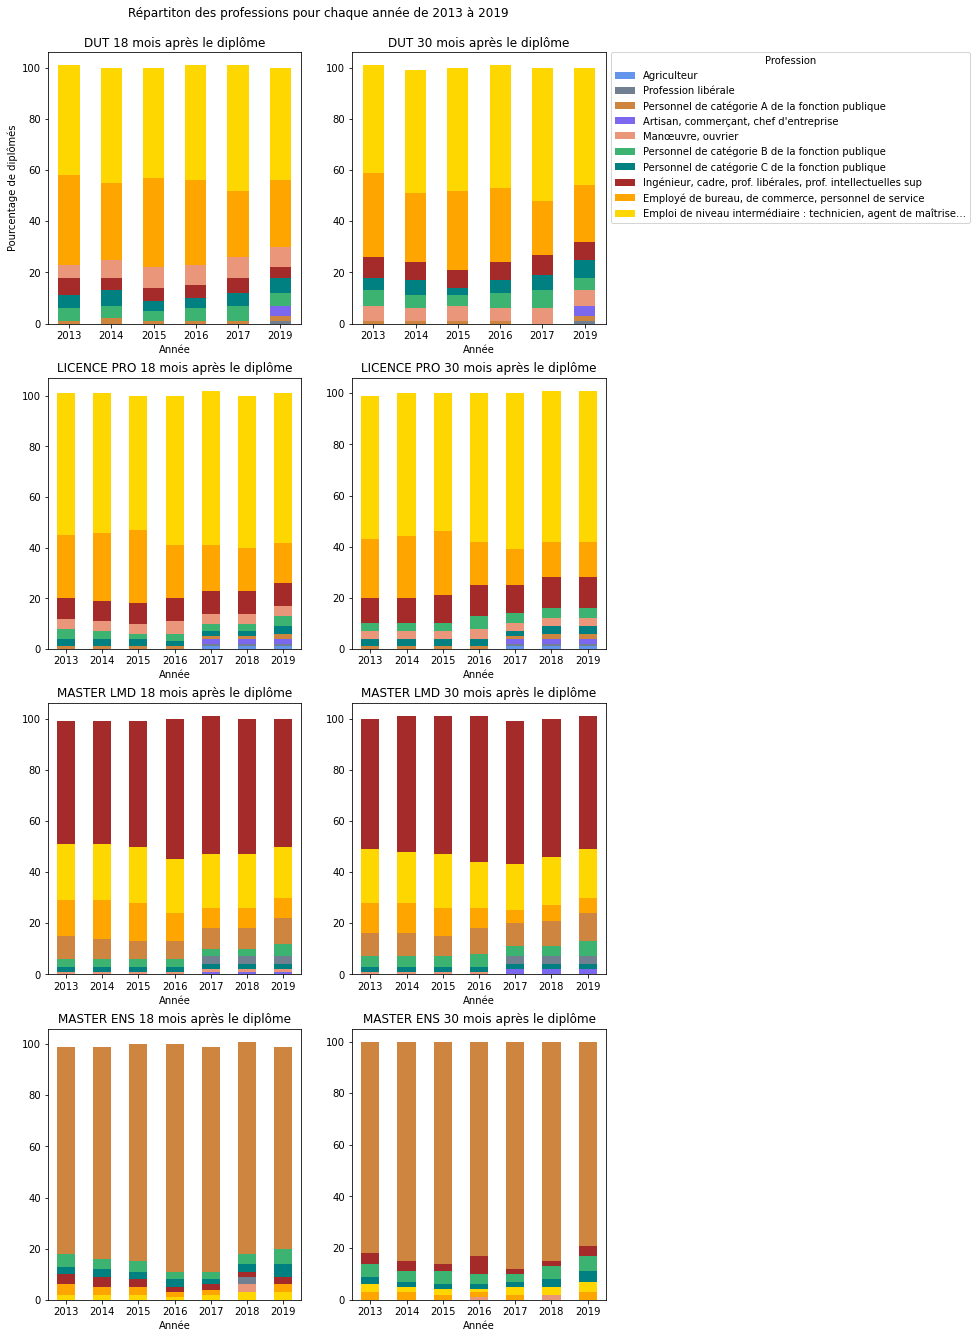
\includegraphics[width=1\textwidth]{../graphs/repartition_professions_situation.png}
	\captionof{figure}{\textbf{Répartition des professions à 18 et 30 mois après l'obtention du diplôme}}
\end{figure}

\section{Proportion des secteurs d'activité}

\begin{figure}[H]
	\centering
	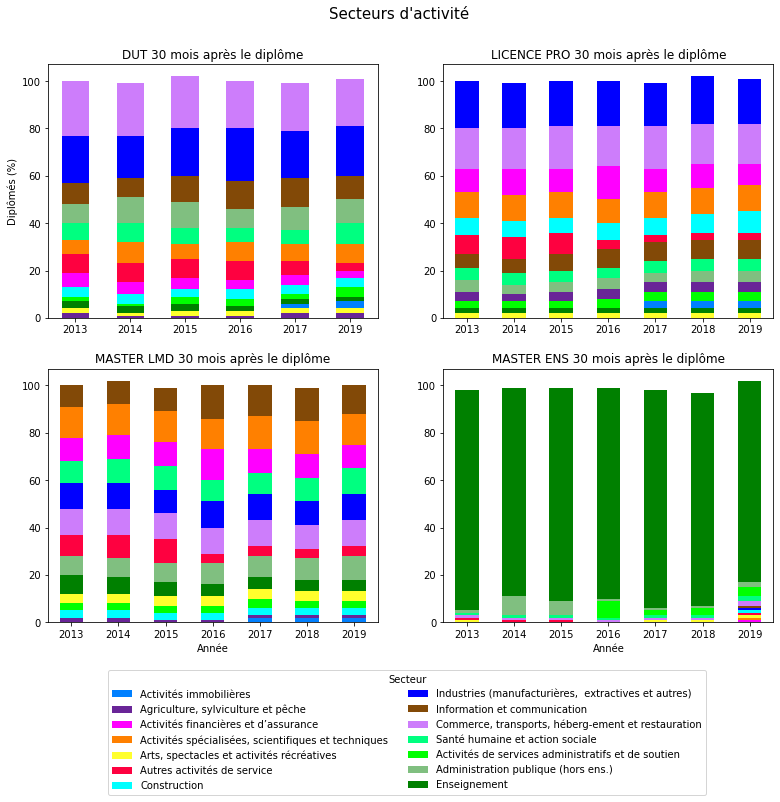
\includegraphics[width=1\textwidth]{../graphs/repartition_secteurs_situation.png}
	\captionof{figure}{\textbf{Répartition des secteurs à 18 et 30 mois après l'obtention du diplôme}}
\end{figure}


\end{document}